\textbf{Теорема о продолжении до границы ограниченной области.}
\newline Пусть $\vec{f}(x, \vec{y})$ определена и удовлетворяет условиям теоремы о существовании и единственности решения задачи
Коши на замыкании ограниченной области $G \subset \R^{n+1}$, тогда любое решение задачи Коши
\begin{equation*}
    \begin{cases}
    \vec{y'}=\vec{f}(x,\vec{y})\\
    \vec{y}(x_0)=\vec{y_0}
    \end{cases}
\end{equation*}
можно продолжить в обе стороны до выхода на $\Gamma = \partial G$, т.е. можно доопределить $\vec{y}(x)$ на некоторый $ [x_0 - \delta, x_0 + \delta] \subseteq [a, b]$, причём $(a, \vec{y}(a)),\;(b, \vec{y}(b)) \in \Gamma$.

\Proof Воспользуемся обозначениями из доказательства теоремы о существовании и единственности (а также цилиндрической метрикой):
\begin{align*}
    \overline{H_{r}} (x_0) &= \{ (x, \vec{y}) \in G: x \in [x_0 - \delta_r, x_0 + \delta_r] \;\; \text{и} \;\; |\vec{y} - \vec{y_0}| \leqslant r \} \subset G. \qquad \qquad \delta_r = \mathlarger{\frac{r}{M + Lr}} \\
    \rho((x_1,&\vec{y_1}),(x_2, \vec{y_2})) = max\{|x_1 - x_2|, |\vec{y_1} - \vec{y_2}|\}
\end{align*}
Введём также расстояние от точки $p$ до множества $M$: $\rho(p, M) = \inf\limits_{q\in M}\rho(p, q).$

Наконец, определим $\delta_0$ и $r_0$ как значения $\delta_r$ и $r$ для точки $p_0 = (x_0, \vec{y_0})$, для которых
выполнено $\max\{\delta_0, r_0\} = \rho(p_0, \Gamma)$. (Это возможно, поскольку $\delta(r)$ и $r(\delta)$ являются строго
возрастающими непрерывными функциями.)

Рассмотрим $x_1 = x_0 + \delta_0$ и $\vec{y_1} = \vec{y}(x_1)$. Обозначим $p_1=(x_1,\vec{y_1})$.
\begin{itemize}
    \item Если $p_1 \in \Gamma$, то продолжение вправо не требуется 
    \begin{figure}[h]
    \hspace{5.2ex}
    \begin{minipage}[h]{0.5\linewidth}
    \item Если $p_1 \notin \Gamma$, то $p_1$ -- внутренняя точка,
а значит, в ней $\exists!$ решение ЗК, причём оно совпадает с
решением для $p_0$ на $[x_0, x_0 + \delta_0]\; \cap \; [x_1 - \delta_1, x_1]$ (где $\delta_1$ и $r_1$, опять же, берутся из теоремы и
условия на расстояние до границы). \newline Аналогично определяем $p_2$, и т. д.
    \end{minipage}
    \hfill
    \hspace{-4ex} \begin{minipage}[h]{0.5\linewidth}
    \center{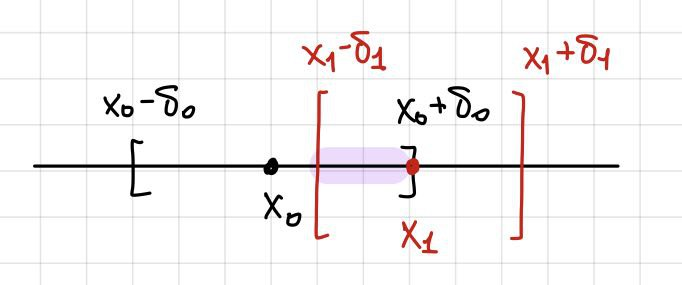
\includegraphics[width=0.8\linewidth]{images/Koshi_prodol.jpg}}
    \end{minipage}
\end{figure}
\end{itemize}
\vspace{-2ex}
Полученная последовательность $\{p_k\}$ монотонно возрастает по $x$ и ограничена точками из $\Gamma$. \newline Следовательно, по теореме Вейерштрасса существует
$b = \lim\limits_{k\to\infty}x_k=x_0 + \sum\limits_{k=0}^{\infty}\delta_k$, при этом $\delta_k > 0$. \newline Объединение решений задач Коши
является функцией, определённой на $\bigcup\limits_{k=1}^{\infty}[x_0, x_k] = [x_0,b)$. \newline
Зафиксируем $\varepsilon > 0$ и рассмотрим
$\alpha, \beta \in [b - \varepsilon, b)$. Заметим, что
\begin{equation*}
    |\vec{y}(\beta)-\vec{y}(\alpha)| = \bigg|\int\limits_{\alpha}^{\beta}\vec{f}(\tau, \vec{y}(\tau))d\tau\bigg| \; \leqslant \int\limits_{\alpha}^{\beta}\Big|\vec{f}(\tau, \vec{y}(\tau))\Big|d\tau \leqslant M\varepsilon
\end{equation*}
Значит, по критерию Коши существует $y^* = \lim\limits_{x\to b-0}\vec{y}(x)$.  Пусть $p^* = (b, \vec{y^*})$. 
\begin{equation*}
    0 \leqslant \rho(p_k,\Gamma) = \max\{\delta_k, r_k\} \to 0 \;\;\;\; (\text{так как $\delta_k\to 0$ и следовательно $r_k\to 0$})
\end{equation*}
Значит $\rho(p^*, \Gamma) = \lim\limits_{k\to\infty}\rho(p_k, \Gamma) = 0 \quad \Rightarrow \quad p^*\in\Gamma$
\begin{equation*}
    \frac{\vec{y}(b) - \vec{y}(b-\varepsilon)}{\varepsilon} = \int\limits_{b-\varepsilon}^{b} \frac{1}{\varepsilon}\vec{f}(\tau, \vec{y}(\tau))d\tau \stackrel{(*)}{=} \frac{\vec{f}(\xi, \vec{y}(\xi))\cdot \varepsilon}{\varepsilon} = \vec{f}(\xi, \vec{y}(\xi)) \stackrel{\varepsilon\to 0}{\longrightarrow} \vec{f}(b, \vec{y}(b))
\end{equation*}
При этом $\vec{f}$ -- непрерывна всюду вплоть до границы $G \;\; \Rightarrow \;\; \vec{f} \in C(p^*)$. Тогда можем сделать переход $(*)$ по интегральной теореме о среднем, где $\xi \in [b - \varepsilon, b]$.

Таким образом мы успешно продолжили вправо, аналогично можно продолжить и влево
\begin{center}
    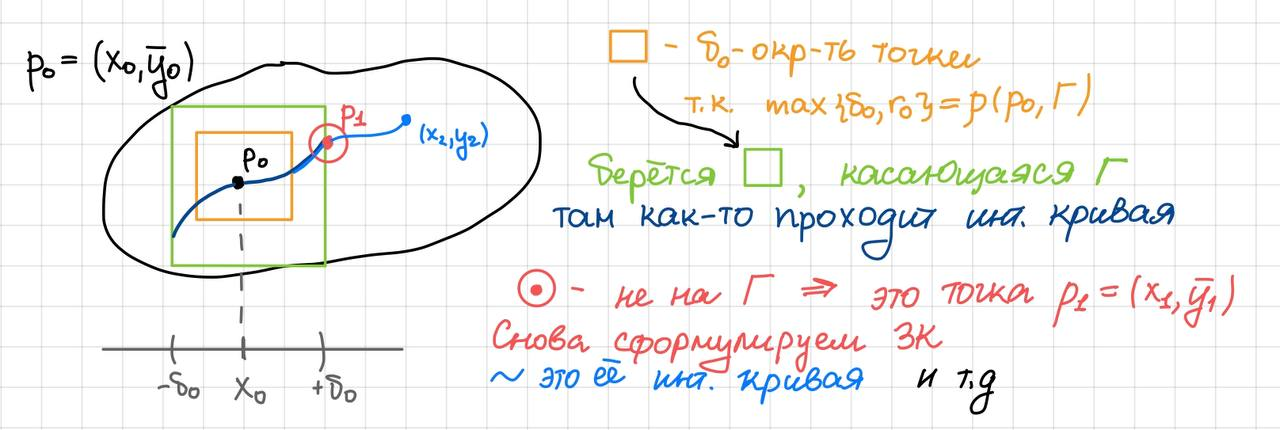
\includegraphics[width=0.8\linewidth]{images/KoshiMainjpg.jpg} \quad \EndProof
\end{center}
\textbf{Следствие.} Пусть $G$ -- замкнутая неограниченная область в $\R^{n+1}$, для которой выполнено $\forall c, d \in \R \;\; (c < d \Rightarrow \; G_{cd}$ ограниченно), где $G_{cd} = \{(x, \vec{y}) \in G \;|\; x \in [c, d]\}$, и $\vec{f}(x, \vec{y})$
удовлетворяет условиям теоремы существования и единственности решения задачи Коши
в $G$, тогда решение в любой точке из $G$ можно продолжить до границы $G$ или сколь угодно
большого (по модулю) значения $x$.
\newline \begin{figure}[h]
    \hspace{-4ex} \begin{minipage}[h]{0.5\linewidth}
    \center{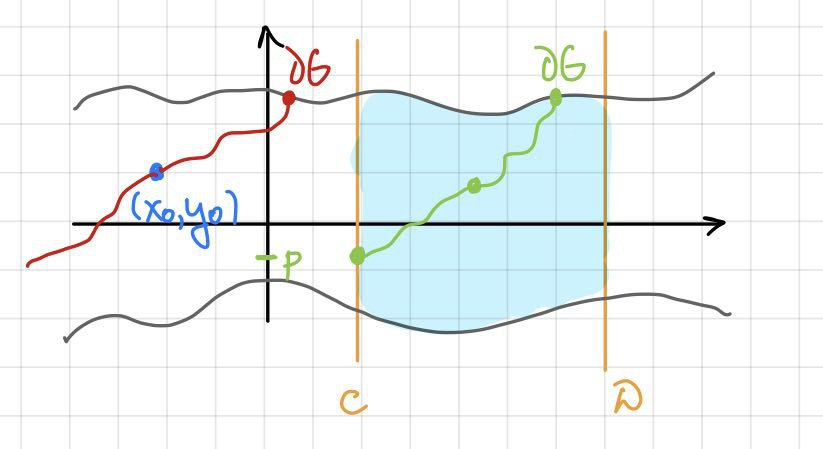
\includegraphics[width=0.8\linewidth]{images/Koshi_sl.jpg}}
    \end{minipage}
    \hfill
    \begin{minipage}[h]{0.6\linewidth}
    \Proof Заметим, что для произвольного отрезка $[c, d]:$ \newline $\; x_0 \in [c,d]$  -- решение задачи Коши на этом отрезке \newline(оно существует по предыдущей теореме). \newlineЕсли интегральная кривая
решения не “дошла” \newlineдо границы $G$, то увеличиваем $d$ \newline и повторяем процесс.\quad \EndProof
    \end{minipage}
\end{figure}
\bigbreak
\textbf{Лемма Гронуолла (усиленная)}. Пусть на промежутке $I$ функция $\varphi(x)$ неотрицательна, непрерывна и удовлетворяет неравенству:
\begin{equation*}
    \varphi(x)\leqslant A + B\Bigg|\int\limits_{x_0}^{x}\varphi(\tau)d\tau\Bigg|+C|x-x_0|
\end{equation*}
где $A, C \geqslant 0$, $B > 0$, $x, x_0 \in I$ и $x \neq x_0$, тогда
\begin{equation*}
    \forall x \in I \quad \varphi(x) \leqslant Ae^{B|x-x_0|}+ \frac{C}{B}\Big(e^{B|x-x_0|} - 1\Big)
\end{equation*}
\Proof Пусть $x > x_0$ (второй случай технически аналогичен). Введём $\Phi(x) =
\int\limits_{x_0}^{x} \varphi(t) dt $, тогда
\begin{equation*}
    0 \leqslant \Phi'(x) = \varphi(x) \leqslant A + B\Phi(x) + C(x-x_0)
\end{equation*}
Домножим обе части на $e^{-B(x-x_0)}$, тогда получим
\begin{align*}
    \Phi'(x)e^{-B(x-x_0)} \leqslant Ae^{-B(x-x_0)} + B\Phi(x)e^{-B(x-x_0)} + C(x-x_0)e^{-B(x-x_0)} \\
    \Phi'(x)e^{-B(x-x_0)} - B\Phi(x)e^{-B(x-x_0)} \leqslant Ae^{-B(x-x_0)} + C(x-x_0)e^{-B(x-x_0)} \\
    \Big(\Phi(x)e^{-B(x-x_0)}\Big)' \leqslant Ae^{-B(x-x_0)} + C(x-x_0)e^{-B(x-x_0)} \\
    \int\limits_{x_0}^x \Big(\Phi(t)e^{-B(t-x_0)}\Big)'dt \leqslant \int\limits_{x_0}^x\Big(Ae^{-B(t-x_0)} + C(t-x_0)e^{-B(t-x_0)}\Big)dt
\end{align*}
т.к. $\Phi(x_0)=0$, то получаем:
\begin{align*}
    \Phi(x)e^{-B(x-x_0)} \leqslant -\frac{A}{B}e^{-B(x-x_0)}\Big|_{x_0}^{x} -\frac{C}{B}(x-x_0)e^{-B(x-x_0)} - \frac{C}{B^2}e^{-B(x-x_0)}\Big|_{x_0}^{x} \\
    \Phi(x)e^{-B(x-x_0)} \leqslant -\frac{A}{B}e^{-B(x-x_0)} + \frac{A}{B} -\frac{C}{B}(x-x_0)e^{-B(x-x_0)} - \frac{C}{B^2}e^{-B(x-x_0)} + \frac{C}{B^2}
\end{align*}
Домножим обе части на $e^{B(x-x_0)}$, тогда получим
\begin{align*}
    \Phi(x)&\leqslant -\frac{A}{B} + \frac{A}{B}e^{B(x-x_0)} -\frac{C}{B}(x-x_0) - \frac{C}{B^2} + \frac{C}{B^2}e^{B(x-x_0)}
\end{align*}
Подставим полученную оценку в неравенство $\varphi(x) \leq A+B\Phi(x)+C(x-x_0)$
\begin{align*}
    \varphi(x) &\leqslant Ae^{B(x-x_0)} + \frac{C}{B}e^{B(x-x_0)} - \frac{C}{B}\\
    \varphi(x) &\leqslant Ae^{B|x-x_0|}+ \frac{C}{B}\Big(e^{B|x-x_0|} - 1\Big) \text{\;\; \EndProof}
\end{align*}

\textbf{Теорема о продолжении на весь заданный интервал.}
\newline Пусть вектор-функция
$\vec{f}(x, \vec{y})$ удовлетворяет условию теоремы о существовании и единственности решения задачи Коши на области $G$: $\alpha < x < \beta$, и $\vec{y} \in \R^n$ ($\alpha$ и $\beta$ могут быть бесконечными). Кроме того, $|\vec{f}(x,\vec{y})|\;\leqslant b(x)\cdot |\vec{y}| + c(x)$, где $b(x)$ и $c(x)$ -- непрерывные на $(\alpha, \beta)$ функции. В таком случае
каждое решение системы $\vec{y'}(x) = \vec{f}(x, \vec{y})$, проходящее в области $G$, можно продолжить на
весь интервал $(\alpha, \beta)$.
\bigbreak
\Proof Пусть некоторое решение системы определено на $[\alpha_1, \beta_1]$. \newline Определим $B=\max\limits_{[\alpha_1,\beta_1]}|b(x)|$ и $C=\max\limits_{[\alpha_1,\beta_1]}|c(x)|$. Тогда  $|\vec{y'}(x)| \;= |\vec{f}(x,\vec{y})|\;\leqslant B |\vec{y}| + C$ и
\begin{align*}
    |\vec{y}(x)| &\;\leqslant |\vec{y_0}|\; + \Bigg|\int\limits_{x_0}^x\vec{f}(t,\vec{y})dt\Bigg| \\
    &\;\leqslant |\vec{y_0}|\; + \int\limits_{x_0}^x\Big|\vec{f}(t,\vec{y})\Big|dt \\
    &\;\leqslant |\vec{y_0}|\; + B \int\limits_{x_0}^x|\vec{y}|dt + C(x-x_0)
\end{align*}
По лемме Гронуолла получаем
\begin{equation*}
    |\vec{y}(x)| \;\leqslant \underbrace{ |\vec{y_0}|\,\cdot\, e^{B|x-x_0|}+ \frac{C}{B}\Big(e^{B|x-x_0|} - 1\Big)}_{(*)}
\end{equation*}
Обозначит $M = \max\limits_{[\alpha_1,\beta_1]} |*|$. Пусть $G_1\;=\;\{(x,\vec{y})\in\R^{n+1} \; :\; \alpha_1\leqslant x\leqslant \beta_1 \text{ и }|\vec{y}|\leqslant M + 1\}$

\noindent По ранее доказанной теореме продолжим решение до границы $G_1$ (зелёная область на картинке).
 
\noindent Повторяя данный процесс, получим последовательность $\{[\alpha_i, \beta_i]\}$, для которой верно $\bigcup[\alpha_i, \beta_i] = (\alpha, \beta)$. Искомое решение также получается объединением.
\begin{center}
    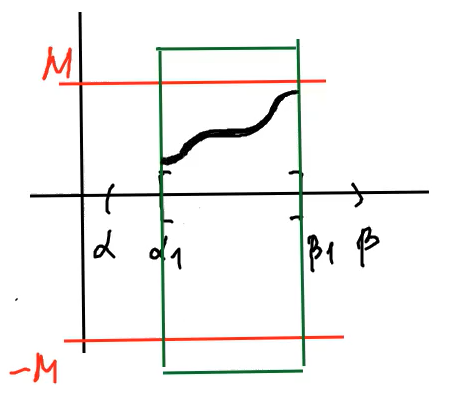
\includegraphics[width=0.35\linewidth]{images/LL.png}
    \qquad \EndProof
\end{center}
